% Options for packages loaded elsewhere
\PassOptionsToPackage{unicode}{hyperref}
\PassOptionsToPackage{hyphens}{url}
%
\documentclass[
  letterpaper,
  ignorenonframetext,
  aspectratio=43,
  handout,
  12pt]{beamer}
\usepackage{pgfpages}
\setbeamertemplate{caption}[numbered]
\setbeamertemplate{caption label separator}{: }
\setbeamercolor{caption name}{fg=normal text.fg}
\beamertemplatenavigationsymbolsempty
% Prevent slide breaks in the middle of a paragraph
\widowpenalties 1 10000
\raggedbottom
\setbeamertemplate{part page}{
  \centering
  \begin{beamercolorbox}[sep=16pt,center]{part title}
    \usebeamerfont{part title}\insertpart\par
  \end{beamercolorbox}
}
\setbeamertemplate{section page}{
  \centering
  \begin{beamercolorbox}[sep=12pt,center]{part title}
    \usebeamerfont{section title}\insertsection\par
  \end{beamercolorbox}
}
\setbeamertemplate{subsection page}{
  \centering
  \begin{beamercolorbox}[sep=8pt,center]{part title}
    \usebeamerfont{subsection title}\insertsubsection\par
  \end{beamercolorbox}
}
\AtBeginPart{
  \frame{\partpage}
}
\AtBeginSection{
  \ifbibliography
  \else
    \frame{\sectionpage}
  \fi
}
\AtBeginSubsection{
  \frame{\subsectionpage}
}
\usepackage{amsmath,amssymb}
\usepackage{lmodern}
\usepackage{ifxetex,ifluatex}
\ifnum 0\ifxetex 1\fi\ifluatex 1\fi=0 % if pdftex
  \usepackage[T1]{fontenc}
  \usepackage[utf8]{inputenc}
  \usepackage{textcomp} % provide euro and other symbols
\else % if luatex or xetex
  \usepackage{unicode-math}
  \defaultfontfeatures{Scale=MatchLowercase}
  \defaultfontfeatures[\rmfamily]{Ligatures=TeX,Scale=1}
\fi
\usetheme[]{metropolis}
% Use upquote if available, for straight quotes in verbatim environments
\IfFileExists{upquote.sty}{\usepackage{upquote}}{}
\IfFileExists{microtype.sty}{% use microtype if available
  \usepackage[]{microtype}
  \UseMicrotypeSet[protrusion]{basicmath} % disable protrusion for tt fonts
}{}
\makeatletter
\@ifundefined{KOMAClassName}{% if non-KOMA class
  \IfFileExists{parskip.sty}{%
    \usepackage{parskip}
  }{% else
    \setlength{\parindent}{0pt}
    \setlength{\parskip}{6pt plus 2pt minus 1pt}}
}{% if KOMA class
  \KOMAoptions{parskip=half}}
\makeatother
\usepackage{xcolor}
\IfFileExists{xurl.sty}{\usepackage{xurl}}{} % add URL line breaks if available
\IfFileExists{bookmark.sty}{\usepackage{bookmark}}{\usepackage{hyperref}}
\hypersetup{
  hidelinks,
  pdfcreator={LaTeX via pandoc}}
\urlstyle{same} % disable monospaced font for URLs
\newif\ifbibliography
\usepackage{graphicx}
\makeatletter
\def\maxwidth{\ifdim\Gin@nat@width>\linewidth\linewidth\else\Gin@nat@width\fi}
\def\maxheight{\ifdim\Gin@nat@height>\textheight\textheight\else\Gin@nat@height\fi}
\makeatother
% Scale images if necessary, so that they will not overflow the page
% margins by default, and it is still possible to overwrite the defaults
% using explicit options in \includegraphics[width, height, ...]{}
\setkeys{Gin}{width=\maxwidth,height=\maxheight,keepaspectratio}
% Set default figure placement to htbp
\makeatletter
\def\fps@figure{htbp}
\makeatother
% Make links footnotes instead of hotlinks:
\DeclareRobustCommand{\href}[2]{#2\footnote{\url{#1}}}
\setlength{\emergencystretch}{3em} % prevent overfull lines
\providecommand{\tightlist}{%
  \setlength{\itemsep}{0pt}\setlength{\parskip}{0pt}}
\setcounter{secnumdepth}{-\maxdimen} % remove section numbering
\usepackage{pgfpages}
\pgfpagesuselayout{2 on 1}
\providecommand{\tightlist}{%
\setlength{\itemsep}{0pt}\setlength{\parskip}{0pt}}
\makeatletter
\makeatother
\let\Oldincludegraphics\includegraphics
\renewcommand{\includegraphics}[2][]{\Oldincludegraphics[width=\textwidth,height=0.7\textheight,keepaspectratio]{#2}}
\ifluatex
  \usepackage{selnolig}  % disable illegal ligatures
\fi

\author{}
\date{}

\begin{document}

\begin{frame}{Mechanics of Materials}
\protect\hypertarget{mechanics-of-materials}{}
Lecture 8 - Axial Load, Torsion

Dr.~Nicholas Smith

Wichita State University, Department of Aerospace Engineering

1 March, 2021
\end{frame}

\begin{frame}{schedule}
\protect\hypertarget{schedule}{}
\begin{itemize}
\tightlist
\item
  1 Mar - Axial Load
\item
  3 Mar - Torsion
\item
  5 Mar - Homework 3 Due
\item
  8 Mar - Torsion
\item
  10 Mar - Bending
\item
  12 Mar - Homework 4 Due, Homework 3 Self-grade due
\end{itemize}
\end{frame}

\begin{frame}{outline}
\protect\hypertarget{outline}{}
\begin{itemize}
\tightlist
\item
  superposition
\item
  statically indeterminate
\item
  force method
\item
  thermal stress
\item
  torsion
\end{itemize}
\end{frame}

\hypertarget{superposition}{%
\section{superposition}\label{superposition}}

\begin{frame}{superposition}
\protect\hypertarget{superposition-1}{}
\begin{itemize}
\tightlist
\item
  Some problems are too complicated to solve all at once
\item
  Instead, we break them up into two simpler problems
\item
  Each ``sub-problem'' must still satisfy equilibrium
\item
  Problem must be linear and the deformation should be small enough that
  it does not cause moment-equilibrium issues
\end{itemize}
\end{frame}

\hypertarget{statically-indeterminate}{%
\section{statically indeterminate}\label{statically-indeterminate}}

\begin{frame}{statically indeterminate}
\protect\hypertarget{statically-indeterminate-1}{}
\begin{itemize}
\tightlist
\item
  There are many problems that are at least slightly over-constrained
\item
  While this is common engineering practice, it creates too many
  variables for statics analysis
\item
  These problems are called ``statically indeterminate''
\end{itemize}
\end{frame}

\begin{frame}{statically indeterminate}
\protect\hypertarget{statically-indeterminate-2}{}
\begin{itemize}
\tightlist
\item
  One extra equation we can use is called ``compatibility'' or the
  ``kinematic condition''
\item
  We know that at the displacement must be equal on both sides of any
  arbitrary section we make in a member
\item
  We can separate a member into two parts, then use compatibility to
  relate the two unknown forces
\end{itemize}
\end{frame}

\begin{frame}{statically indeterminate}
\protect\hypertarget{statically-indeterminate-3}{}
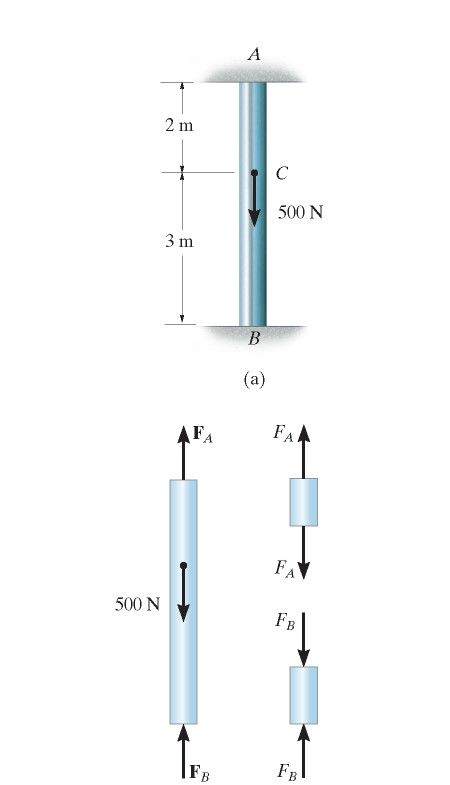
\includegraphics{../images/statically-indeterminate.jpg}
\end{frame}

\begin{frame}{example 4.7}
\protect\hypertarget{example-4.7}{}
\begin{columns}[T]
\begin{column}{0.5\textwidth}
\begin{figure}
\centering
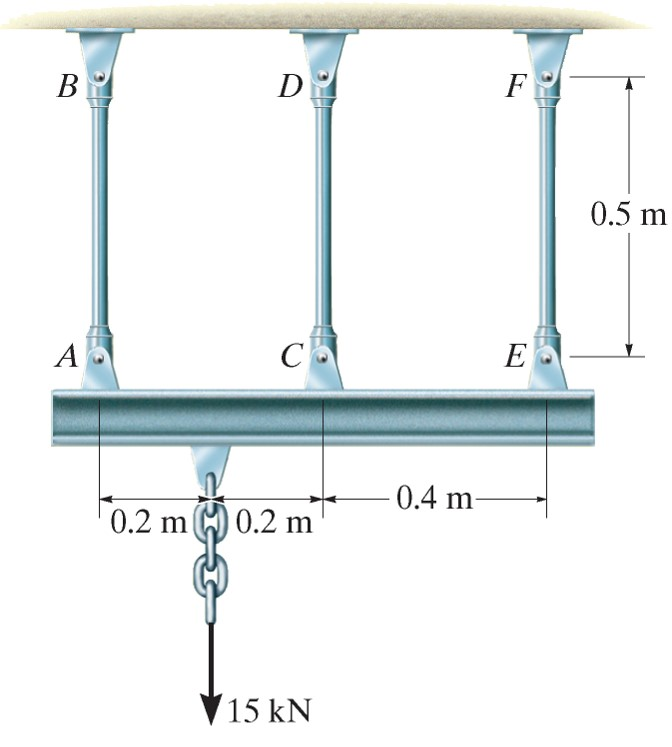
\includegraphics{../images/example-4-7.jpg}
\caption{A 0.8 m long rigid horizontal bar is supported by hanging from
3 vertical rods. Rod AB supports the left end, rod CD supports the
middle and rod EF supports the right end. A 15 kN load is applied 0.2 m
from the left end.}
\end{figure}
\end{column}

\begin{column}{0.5\textwidth}
Assuming the bottom bar is rigid, find the force developed in each bar.
AB and EF have cross-sectional areas of 50 mm2 while CD has a
cross-sectional area of 30 mm2.
\end{column}
\end{columns}
\end{frame}

\hypertarget{force-method}{%
\section{force method}\label{force-method}}

\begin{frame}{force method}
\protect\hypertarget{force-method-1}{}
\begin{itemize}
\tightlist
\item
  One way to solve statically indeterminate problems is using the
  principle of superposition
\item
  We choose one redundant support and remove it
\item
  We then add it back as a force separately (without the other forces in
  the problem)
\end{itemize}
\end{frame}

\begin{frame}{force method}
\protect\hypertarget{force-method-2}{}
\begin{figure}
\centering
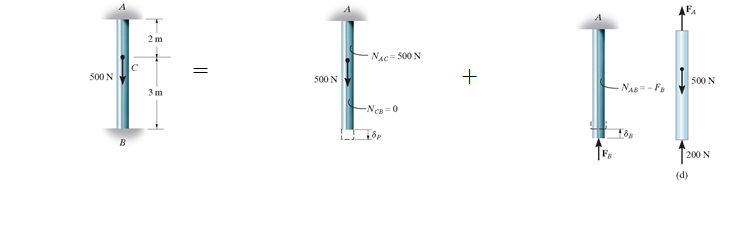
\includegraphics{../images/force-method.png}
\caption{An illustration of the force method, we have the same
statically indeterminate problem as before, a 5 m long,
vertically-oriented bar is fixed at both ends, with a 500 N downward
load applied 2 m from the top. We set this equivalent to a bar with the
same load, but no support on the bottom end. We then add a force which
will provide enough displacement to cancel out the displacement
introduced by removing the load.}
\end{figure}
\end{frame}

\begin{frame}{force method}
\protect\hypertarget{force-method-3}{}
\begin{itemize}
\tightlist
\item
  We connect the two problems by requiring that the displacement in both
  frames adds to 0 to meet the support requirements
\item
  This is referred to as the equation of compatibility
\end{itemize}
\end{frame}

\begin{frame}{procedure}
\protect\hypertarget{procedure}{}
\begin{itemize}
\tightlist
\item
  Choose one support as redundant, write the equation of compatibility
\item
  Express the external load and redundant displacements in terms of
  load-displacement relationship
\item
  Draw free body diagrams and use the equations of equilibrium to solve
\end{itemize}
\end{frame}

\begin{frame}{example 4.9}
\protect\hypertarget{example-4.9}{}
\begin{figure}
\centering
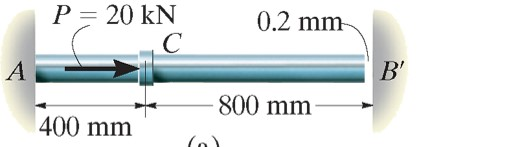
\includegraphics{../images/example-4-9.jpg}
\caption{A 1200 mm long horizontal rod is fixed at its left end and has
a fixed support 0.2 mm away from its right end. A 20 kN load is applied
to the right 400 mm away from its left end.}
\end{figure}

The steel rod shown has a diameter of 10 mm. Determine the reactions at
A and B'.
\end{frame}

\hypertarget{thermal-stress}{%
\section{thermal stress}\label{thermal-stress}}

\begin{frame}{thermal stress}
\protect\hypertarget{thermal-stress-1}{}
\begin{itemize}
\tightlist
\item
  A change in temperature cases a material to either expand or contract
\item
  For most materials this is linear and can be described using the
  coefficient of linear expansion
\end{itemize}

\[\delta_T = \alpha \Delta T L\]
\end{frame}

\begin{frame}{thermal stress}
\protect\hypertarget{thermal-stress-2}{}
\begin{itemize}
\tightlist
\item
  When a body is free to expand, the deformation can be readily
  calculated using
\item
  If it is not free to expand, however, thermal stresses develop
\item
  We can use the force method described previously to find the thermal
  stresses developed
\end{itemize}
\end{frame}

\begin{frame}{example 4.12}
\protect\hypertarget{example-4.12}{}
\begin{columns}[T]
\begin{column}{0.5\textwidth}
\begin{figure}
\centering
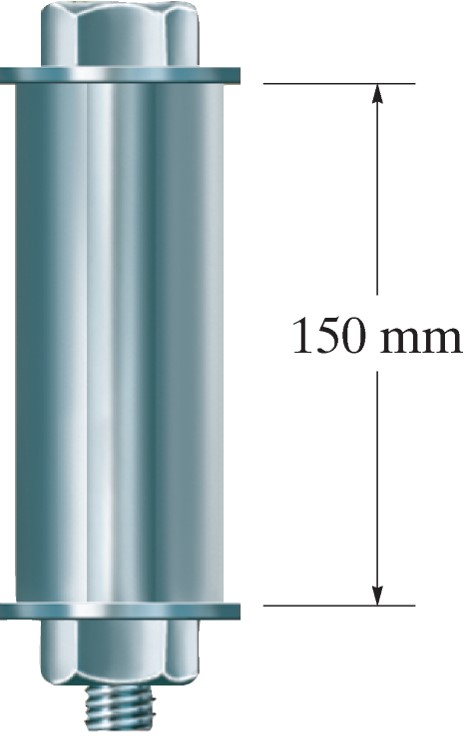
\includegraphics{../images/example-4-12.jpg}
\caption{An aluminum tube used as a sleeve for a steel bolt. The tube is
150 mm long.}
\end{figure}
\end{column}

\begin{column}{0.5\textwidth}
An aluminum tube with cross-section of 600 mm2 is used as a sleeve for a
steel bolt with cross-sectional area of 400 mm2. When T=15 degrees
Celsius there is negligible force and a snug fit, find the force in the
bolt and sleeve when T=80 degrees Celsius.
\end{column}
\end{columns}
\end{frame}

\hypertarget{torsion}{%
\section{torsion}\label{torsion}}

\begin{frame}{torsion}
\protect\hypertarget{torsion-1}{}
\begin{itemize}
\tightlist
\item
  Torque is a moment that tends to twist a member about its axis
\item
  For small deformation problems, we assume that the length and radius
  do not change significantly under torsion
\item
  The primary deformation we are concerned with in torsion is the angle
  of twist, denoted with \$\phi\$
\end{itemize}
\end{frame}

\begin{frame}{shear}
\protect\hypertarget{shear}{}
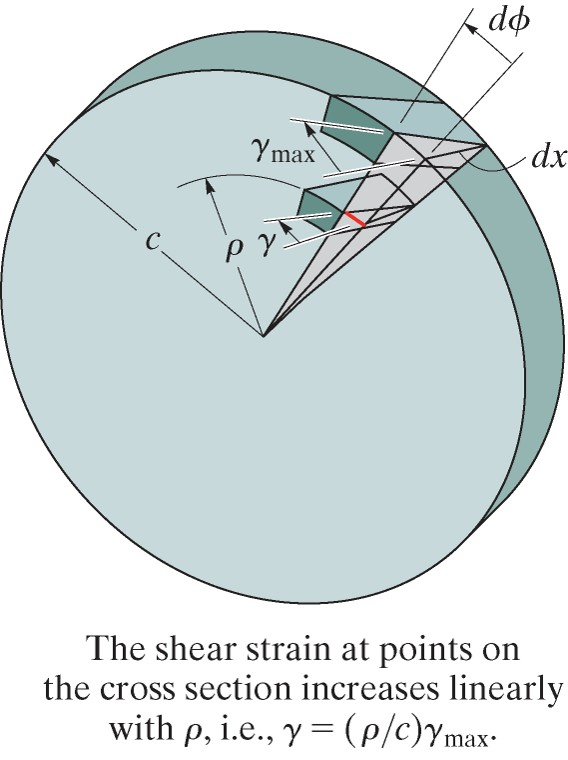
\includegraphics{../images/torsion-disk.jpg}
\end{frame}

\begin{frame}{torsion formula}
\protect\hypertarget{torsion-formula}{}
\begin{itemize}
\tightlist
\item
  For a linearly elastic material, Hooke's Law in shear will hold
  (\(\tau = G \gamma\))
\item
  This means that, like shear strain, shear stress will vary linearly
  along the radius
\end{itemize}
\end{frame}

\begin{frame}{torsion formula}
\protect\hypertarget{torsion-formula-1}{}
\begin{itemize}
\tightlist
\item
  We can find the total force on an element, \emph{dA} by multiplying
  the shear stress by the area
\end{itemize}

\[ dF = \tau dA\]

\begin{itemize}
\tightlist
\item
  The torque (\(dT = \rho dF\)) produced by this force is then
\end{itemize}

\[dT = \rho(\tau dA)\]
\end{frame}

\begin{frame}{torsion formula}
\protect\hypertarget{torsion-formula-2}{}
\begin{itemize}
\tightlist
\item
  Integrating over the whole cross-section gives
\end{itemize}

\[T = \int_A \rho (\tau dA) = \frac{\tau_{max}}{c} \int_A \rho^2 dA\]

\begin{itemize}
\tightlist
\item
  The integral \(\int_A \rho^2 dA\) is also called the Polar Moment of
  Inertia, \emph{J}, so we can write
\end{itemize}

\[\tau_{max} = \frac{Tc}{J}\]
\end{frame}

\begin{frame}{polar moment of inertia}
\protect\hypertarget{polar-moment-of-inertia}{}
\begin{itemize}
\tightlist
\item
  We know that \(J=\int_A \rho^2 dA\), so we can compute this for some
  common shapes
\item
  For a solid circular cross-section, we have
\end{itemize}

\[J = \int_0^c \rho^2 (2\pi \rho d\rho) = \frac{\pi}{2}c^4\]

\begin{itemize}
\tightlist
\item
  For a circular tube we have
\end{itemize}

\[J = \int_{c_1}^{c_2} \rho^2 (2\pi \rho d\rho) = \frac{\pi}{2}(c_2^4-c_1^4)\]
\end{frame}

\begin{frame}{example 5.1}
\protect\hypertarget{example-5.1}{}
\begin{columns}[T]
\begin{column}{0.5\textwidth}
\begin{figure}
\centering
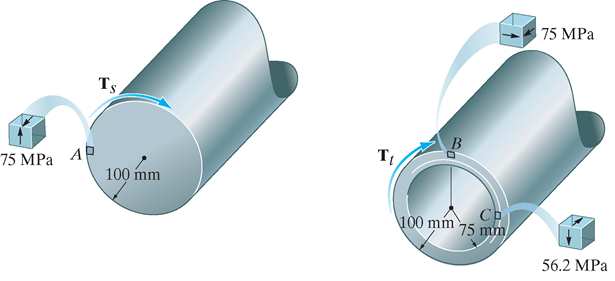
\includegraphics{../images/example-5-1.png}
\caption{On left is a solid 100 mm radius tube, while on the right is a
hollow tube with outer radius of 100 mm and inner radius of 75 mm.
Element A is on the surface of the solid tube on the left, element B is
on the outer surface of the hollow tube on the right and Element C is on
the inner surface of the hollow tube on the right.}
\end{figure}
\end{column}

\begin{column}{0.5\textwidth}
The allowable shear stress is 75 MPa. Determine the maximum torque that
can be applied to each of the cross-sections shown and find the stress
acting on a small element at A, B and C.
\end{column}
\end{columns}
\end{frame}

\end{document}
